\documentclass[a4paper, 10pt,hidelinks]{article}
\usepackage{amsmath}
\usepackage{amssymb}
\usepackage[autostyle]{csquotes}
\usepackage[bookmarks]{hyperref}
\usepackage{xcolor}
\usepackage{graphicx} %to include graphs
\graphicspath{{Figures/}} %path for figures
 \usepackage[left=1in,right=1in,top=1in,bottom=1in,%
            footskip=.25in]{geometry}

\newcommand{\upi}[1]{#1^{(i)}}
\newcommand{\upj}[1]{#1^{(j)}}
\newcommand{\R}{\mathbb{R}}
\newcommand{\ind}[1]{^{(#1)}}
\begin{document}

These are notes based on the Stanford machine learning coursera course by Andrew Ng. They are not final yet and I will update them as I go through the course. These notes will be improved and material from outside the course will be added once I have finished the course.

\section{Linear Regression}
\subsection{Gradient descent}
Let $\theta = (\theta_0, \theta_1, \cdots, \theta_n)$ (column vector) be the parameters and $x^{(i)} = (x^{(i)}_0, \cdots, x^{(i)}_n)$ (also column vector) be the features of the $i$th training example. So we have $n$ features, and also we use $m$ to denote the number of trainig examples.  Our prediction of the outcome variable given the $i$th training example is now given by
\begin{align}
\hat{y}(\upi{x})_{\theta} &= \theta^T \upi{x} \nonumber \\
&= \theta_0 + \theta_1 \upi{x}_1 + \cdots + \theta_n \upi{x}_n
\end{align}
where we chose $x_0 = 1$ so that $\theta_0$ just becomes a constant contribution. 

Generally, we have $m$ samples $(x^{(1)}, y^{(1)}), \cdots, (x^{(m)}, y^{(m)})$ and $n$ features, i.e. 

\begin{equation}
\upi{x} = \begin{pmatrix}
\upi{x_0} \\ 
\upi{x_1} \\ 
\upi{x_2} \\
\vdots \\
\upi{x_n}
\end{pmatrix} \in \R^{n + 1}
\end{equation}
and we define $X \in \R^{m \times n+ 1}$  to be the matrix which contains all the features of all the training examples:
\begin{equation}\label{Eq: Definition X matrix}
X = \begin{pmatrix}
(x^{(1)})^T \\
(x^{(2)})^T \\
\vdots \\
(x^{(m)})^T \\
\end{pmatrix}
\end{equation}
Here $(x^{(1)})^T$ is a row vector, etc.. We can now write the linear model as
\begin{equation}
\hat{y}(X)_{\theta} = X \theta
\end{equation}
which itself is a $m$-dimensional column vector, with each entry the prediction of a given training sample. 

We now define the cost function as 
\begin{equation}\label{Eq: Cost function linear regression}
J(\theta) = \frac{1}{2 m} \sum_{i = 1}^m (\theta^T x^{(i)} - y^{(i)})^2
\end{equation}
where $y^{(i)} = (y^{(i)}_1, y^{(i)}_2, \cdots, y^{(i)}_m)$ are the actual values. This gives the cost for a given training example $\upi{x}$.

For updating our parametes using gradient descent, we use the following rule:
\begin{align}
\theta_k &\rightarrow \theta_k - \alpha \, \partial_{\theta_k} J(\theta) \label{Eq: Theta update rule} \\
&= \theta_k - \alpha \, \frac{1}{m} \sum_{i = 1}^m (\theta^T x^{(i)} - y^{(i)}) \,x_k^{(i)} 
\end{align}
where $\alpha$ is the learning rate. 

Let's write this in a more general form where $\hat{y}_{\theta}(x\ind{i})$ denotes our prediction given $x$ and $\theta$:
\begin{equation}\label{Eq: Unregularized theta update rule}
\theta_k \rightarrow \theta_k - \alpha \, \frac{1}{m} \sum_{i = 1}^m (\hat{y}_{\theta}(x\ind{i}) - y^{(i)}) \,x_k^{(i)} 
\end{equation}


%In vector notation, for when we want to evaluate this on a computer, we can write this (for all $\theta$ simultaneously) as 
%\begin{equation}
%\theta \rightarrow \theta - \alpha/m \,\,\text{Sum} \left[ (X \theta - y).* X \right]
%\end{equation}
%where $.*$ denotes element-wise multiplication and 'Sum' means we want to sum over all the indices. The quantity $(X \theta - y).* X$ is actually a matrix and we want the column-sum. 

\subsection{Feature Scaling}
If one feature takes on much larger values than the other, then with e.g. two features get this very stretched gaussian kind of thing. So very thin in one direction, then it can take ages for gradient descend to reach the minimum. So we need to rescale the features e.g. using mean normalization. This ensures that all features more or less lie in the same range (it doesn't have to be exactly the same, it doesn't have to be exactly between 0 and 1, but just roughly all on the same scale). Mean normalization does the following:
\begin{equation}\label{Eq: Mean norm}
x_i \rightarrow \frac{x_i - \mu_i}{s_i}
\end{equation}
where $\mu_i = 1/n \sum_j x^{(i)}_j$ and $s_i$ is the standard deviation of the $\upi{x}$ vector , $j = 1 \dots n$ ($n$ is the total number of samples we have of this feature $\upi{x}$). 

\subsection{Choosing a learning rate}
Can plot cost function as function of the number of iterations (Figure \ref{Fig: Learning rate figure}). Every iteration of gradient descent we update our parameter vector, and then for the new parameter vector we just evaluate the cost function which is then $J(\theta)$. As we continue with our gradient descent, we move to lower values of the cost so the line decreases and at some point converges (I guess we're not doing stochastic gradient descent because the line is always going down). Can look at this figure when you've done your gradient descent to see whether you converged properly. Can also set a convergent criterion (so e.g. if J changes by less than $10^{-3}$ then you're converged).

Of course a too small learning rate is also not great as the convergence is really slow. Plotting graphs like the ones below is good to see what's going on. Also, \emph{just try a set of different learning rates, e.g. $\alpha = \cdots, 0.001, 0.003, 0.01, 0.03, 0.1, 0.3, \cdots$ and make a plot for each of them. Pick slightly smaller than largest reasonable value.} 

\begin{figure}[h!]
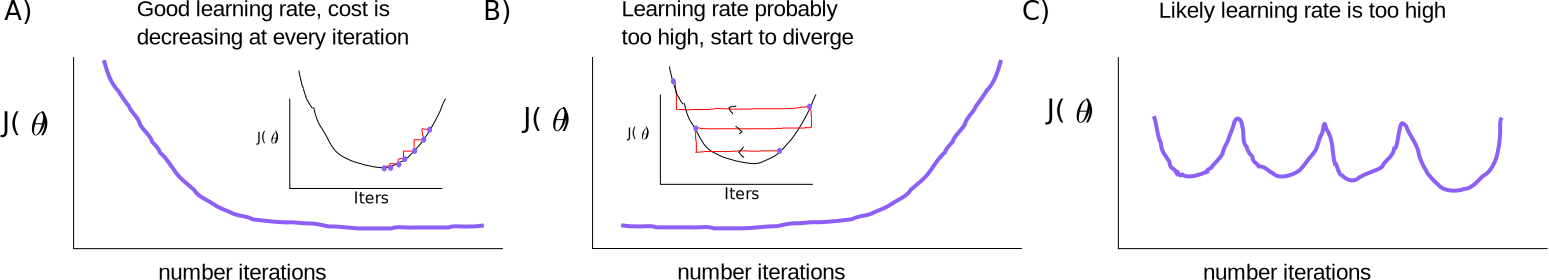
\includegraphics[width=0.94\linewidth]{LearningRate}
\caption{\footnotesize{\textbf{Convergence} {This is determinsitic gradient descent so if done properly the cost should always go down. \textbf{A)} The cost decreases at every iteration and the algorithm is sucessfully approaching the optimum. \textbf{B)} The cost is diverging and it is likely that this is caused by a learning rate that is too large. \textbf{C)} This oscillating behaviour of the cost as function of the number of iterations is also often an indicating of a too large learning rate. }}}
\label{Fig: Learning rate figure}
\end{figure}

\subsection{Choosing features}
It's important to choose good features. Suppose you want to sell a house and you have the width of the house and the depth of the house (so from front to back). Then could say $\hat{y}(x) = \theta_0 + \theta_1 \text{width} + \theta_2 \text{depth}$. But, could make a new feature, e.g. the area, so $A = \text{depth} \times \text{width}$. Then could do $\hat{y}(x) = \theta_0 + \theta_1 A$. This might be a better model.

\subsubsection{Polynomial regression} 
Instead of linear might do something like $\hat{y}(x) = \theta_0 + \theta_1 x  + \theta_2 x^2$ or do a third order one or whatever. Suppose we want our model to depend on the size of a house in a cubic way, so $\hat{y}(x) = \theta_0 + \theta_1 \, (\text{size})  + \theta_2 \, (\text{size})^2  + \theta_3 \, (\text{size})^3$. Then we can just define our features as $x_1 = (\text{size}), x_2 = (\text{size})^2, x_3 = (\text{size})^3$. \emph{So can use linear regression to fit a cubic model to the data.}. Of course can do all kinds of things. It's good to think of what kind of shape you expect the data to be and then select features blah. Note that in this case feature scaling becomes really important, as e.g. $x_3$ in the example is the size cubed so if the size varies over a large scale this $x_3$ will vary over a huge scale, etc.. So be extra careful.

There are algorithms that automatically choose features for you, so that's good :). 


\subsection{Normal equation}
The normal equation lets us solve for the optimal $\theta$, so we don't even have to do gradient descent anymore.

Suppose the cost function is $J(\theta)$ and we have $\theta \in \R^{n + 1}$. Then of course we just do 
\begin{equation}
\partial_{\theta_j} J(\theta) = 0 \quad \forall j
\end{equation}
and solve for all the $\theta_i$. 

In general, we can write $X$ for a matrix of dimension $m \times n+1$, each rows is a training sample and each column is a feature. $X$ was defined previously in Eq. \eqref{Eq: Definition X matrix}. The value of $\theta$ which minimizes the cost function is:
\begin{equation}
\theta  = (X^T X)^{-1} X^T y
\end{equation}
where $y$ is a vector with the actual observed values. So the structure of $X$ is, e.g. if we have 3 features ($x_0$ doesn't count, it is just set to 1) and 4 samples
$X = 
\begin{pmatrix}
x^{(1)}_0 & x^{(1)}_1 & x^{(1)}_2 & x^{(1)}_3 \\
x^{(2)}_0 & x^{(2)}_1 & x^{(2)}_2 & x^{(2)}_3 \\
x^{(3)}_0 & x^{(3)}_1 & x^{(3)}_2 & x^{(3)}_3 \\
x^{(4)}_0 & x^{(4)}_1 & x^{(4)}_2 & x^{(4)}_3
\end{pmatrix}$
and $y = (y^{(1)}, y^{(2)}, y^{(3)}, y^{(4)})$ (a column vector). 

Of course if we use the normal equation we don't have to rescale the features because we're not doing any gradient descent. 

Why don't we just use $\theta = X^{-1} y$? Because $X$ may not be invertible. One can easily show that the normal equation is equivalent to $\theta = X^{-1} y$ while not having to directly take the inverse of $X$. We see that $(X^T X)^{-1}X^T = X^{-1} (X^T)^{-1} X^T = X^{-1}$. It turns out that $X^T X$ is almost always invertible (at least it's a square matrix whereas $X$ may not be).

\subsubsection{When use the normal equation}
With gradient descent, we need to choose the learning rate $\alpha$ which can be annoying. Also, we might need many iterations so it could be slow. 

However, gradient descent works well with a large number of features (say, millions). The normal equation doesn't work well if $n$ is large, it is expensive to calculate $(X^T X)^{-1}$, the matrix $(X^T X)$ is an $n \times n$ matrix. The cost of inverting the matrix goes as $O(n^3)$ so obviously for large $n$ it is very slow to compute this $(X^T X)$ quantity. Gradient descent goes as $O(k n^2)$.

So, for small $n$ use the normal equation, for large $n$ do gradient descent. What is large? If $n = 1000$ still use normal equation, if $n$ is around $10^5$ or $10^6$ then maybe start using gradient descent. 

\subsubsection{What if cannot invert?}
$(X^T X)^{-1}$ might not exist if $(X^T X)$ is not invertible (i.e. it is singular/degenerate). \emph{This apparently is pretty rare}. Even if it's not invertible, you can usually in programming languages still calculate $(X^T X)^{-1}$ numerically somehow. 

If $(X^T X)$ is not invertible this could be caused by redundant features (e.g. one features gives length in meters and another feature gives length in feet, so these are completely dependent). Also, can happen if there are too many features (if e.g. $m \leq n$, try to fit many parameters with just a few training examples) and deleting some might work, or using regularization might work (Section \ref{Sec: Regularization and invertibility}) . Regularization allows you to have a lot of features even with few training examples.

\clearpage
\section{Classification: Logistic Regression}
Examples of classification problems are whether an email is spam or not, whether a tumor is benign or not, whether an image is a cat, dog, horse or goat, etc.. Logistic \emph{regression} is a \emph{classification} algorithm (slightly confusing). 

\subsection{Two classes}
When we have two classes, the true output is either 0 or 1. We will choose our model such that our predictions always lie between 0 and 1. 

We define
\begin{equation}
g(z) = \frac{1}{1 + e^{-z}}
\end{equation}
which is illustrated in Figure \ref{Fig: Logistic regression}A. This is of course just a sigmoid. Now our prediction model is given by 
\begin{equation}
\hat{y}(x)_{\theta} = g(\theta^T x) = \frac{1}{1 + e^{-\theta^T x}}
\end{equation}
Note that $\theta^T x$ doesn't have to be linear, we can define e.g. $x_3 = x_1^2$ (see later examples).

\begin{figure}[h!]
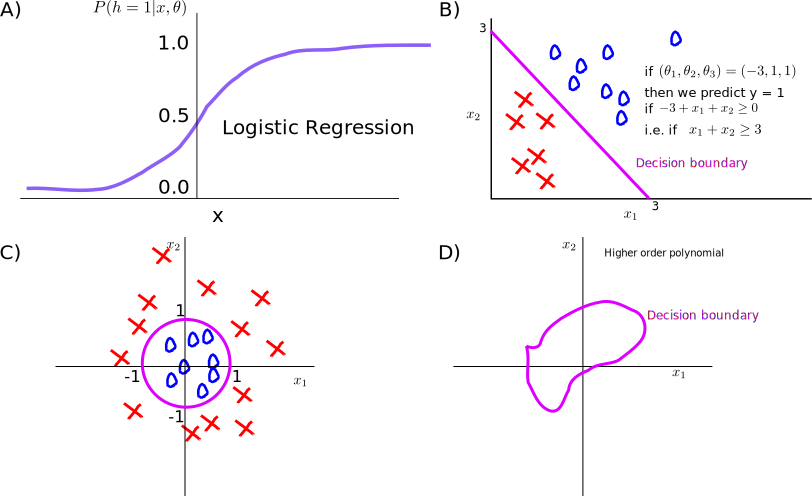
\includegraphics[width=0.9\linewidth]{LogisticRegr}
\caption{\footnotesize{\textbf{Logistic Regression A)} Given some feature input x, we get the logistic thingie as an output and this gives us the probability that the output is 1. \textbf{B)} Decision boundary. }}
\label{Fig: Logistic regression}
\end{figure}

In a simple example for tumor being benign or not, the actual output is either 0 or 1. The output we get can be interpreted as the probability of the output being 1 (which we here choose to be malignant). %The $x$ value here could e.g. be the tumor size (which can take on any value). In our example, the larger the size the more sure we are that the tumor is malignant.

We can now decide to predict an outcome of `1' when $\hat{y} \geq 0.5$. This occurs whenever $\theta^T x \geq 0$.


\subsubsection{Examples}
Suppose we have $\hat{y} = g(\theta_0 + \theta_1 x_1 + \theta_2 x_2)$ with data as shown in Figure \ref{Fig: Logistic regression}B. Using $\theta = (-3, 1, 1)$ works in this exampe as it separates based on the line $x_1 + x_2 \geq 3$. This is exactly a perceptron (see later). The boundry defined by that line is called a \emph{decision boundary}.

We can also say $\hat{y} = g(\theta_0 + \theta_1 x_1 + \theta_2 x_2 + \theta_3 x_1^2 + \theta_4 x^2_2)$ with e.g. $\theta = (-1, 0, 0, 1, 1)$ in which case we will predict `1' if $x_1^2 + x_2^2 \geq 1$, i.e. we can separate the data shown in Figure \ref{Fig: Logistic regression}C. Note that we don't really have to think much about the logistic curve itself, in the end the prediction just depends on whether $\theta^T x \geq 0$. The nice thing about the sigmoid is that we can then get probabilities out of it, so we might predict `1' but we can then say that we're e.g. 70\% sure. 

Higher order polynomials can give more complex decision boundaries (Figure \ref{Fig: Logistic regression}D).

\subsubsection{Fitting parameters}
Given a training set $\{ (x^{(1)}, y^{(1)}), (x\ind{2}, y\ind{2}), \cdots, (x\ind{m}, y\ind{m})\}$ and let $x\ind{i} \in \R^n, y\ind{i} \in \{0, 1\} \, \forall i$, our predictions are given by $\hat{y}(x\ind{i}) = 1/(1 + e^{-\theta^T x\ind{i}})$, then how do we choose the parameters $\theta$?

We write the cost function as $J(\theta) = \frac{1}{m} \sum_{i = 1}^m \text{Cost}(\hat{y}(x\ind{i}), y\ind{i})$ with . Before, with linear regression, we had  $\text{Cost}(\hat{y}(x\ind{i}), y\ind{i}) = \frac{1}{2} (\hat{y}(x\ind{i}) - y\ind{i})^2$. Let's for simplicity write this as $\text{Cost}(\hat{y}(x), y) = \frac{1}{2} (\hat{y}(x) - y)^2$. Can we still use this cost function? No.

When using that square cost function from our linear regression, the actual cost function becomes quite complicated because our $\hat{y}(x)_{\theta}$ is itself a sigmoid. It turns out that the cost function $J(\theta)$, when plugging the sigmoid into the quadratic equation, becomes non-convex. This means we can get stuck in local minima (Figure \ref{Fig: Convex}A, B). 

\begin{figure}[h!]
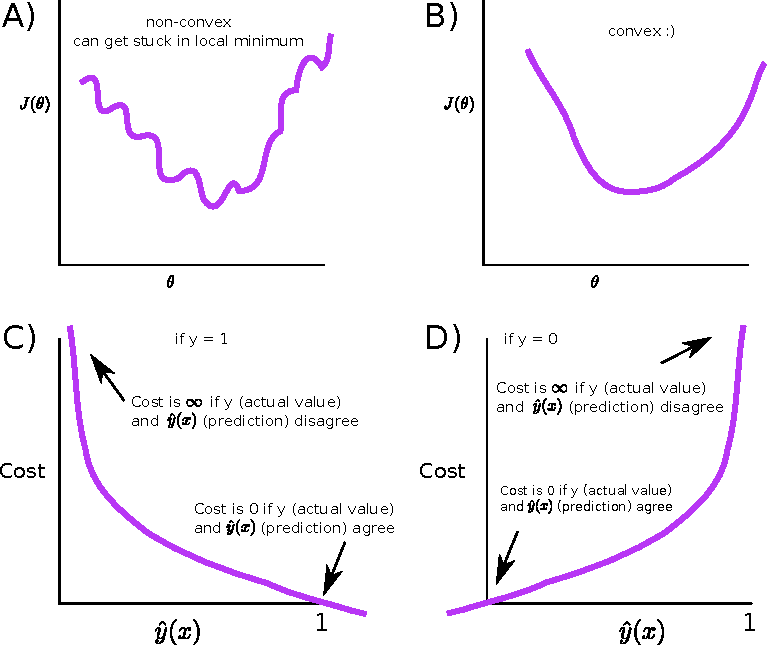
\includegraphics[width=0.8\linewidth]{Convex}
\caption{\footnotesize{\textbf{Pick nice cost function A, B)} If we pick the same cost function as for linear regression, then our overall $J(\theta)$ as a function of $\theta$ will be quite complex and non-convex. This is not what we want, we want a nice looking $J(\theta)$. \textbf{C, D)} When picking the cost function as specified in Eq. \eqref{Eq: Logistic cost function}, we get some nice properties. }}
\label{Fig: Convex}
\end{figure}


What we do, is the following:
\begin{equation}\label{Eq: Logistic cost function}
\text{Cost}(\hat{y}(x), y) = 
\begin{cases}
-\text{log}(\hat{y}(x)) \quad \quad \,\, \;\;\; \;\; \text{if $y$ = 1} \\
-\text{log}(1 - \hat{y}(x)) \quad \quad \text{if $y$ =0}
\end{cases}
\end{equation}
which is shown in Figure \ref{Fig: Convex}C, D. This example was just with a single training example. In general it works as well, the cost function $J(\theta)$ is convex and all is well. Remember that we had assumed that the actual output $y$ is either 0 or 1, so this particular approach we outlined only works if there are 2 classes. % In general, this cost function will be convex and all is well. 

\subsubsection{Simpler cost function}
We can simplify the cost function given in Eq. \eqref{Eq: Logistic cost function}, namely:
\begin{equation}\label{Eq: Logistic final cost function 2 classes}
\text{Cost}(\hat{y}(x), y) = - y\, \text{log}(\hat{y}(x)) - \left[1 - y\right] \text{log} (1 - \hat{y}(x))
\end{equation}
This works of course because $y$ is either 0 or 1 so one of the terms is zero in either case. 

The cost function is therefore:
\begin{equation}\label{Eq: Final Final logistic cost function}
J(\theta) = - \frac{1}{m} \Big[ \sum_{i = 1}^m y\ind{i} \text{log} (\hat{y}(x\ind{i})) + (1 - y\ind{i}) \text{log} \Big(1 - \hat{y}(x\ind{i})\Big) \Big]
\end{equation}

Why this particular function? This cost function can be derived using maximum likelihood estimation, it also has the nice property that it is convex. Basically everyone uses this cost function when fitting logistic regression models. It's not as random as it seems here.

Now what we want of course is find the parameters $\theta$ that minimize $J(\theta)$, and then when we observe a new feature vector we can predict the outcome which is $\hat{y}(x) = 1/(1 + e^{- \theta^T x})$ which is the probability that $y = 1$. Again, we use gradient descent like before. The rule we use is exactly the same as the one in Eq. \eqref{Eq: Theta update rule}, and after computing $\partial_{\theta} J(\theta)$ we get:
\begin{equation}\label{Eq: Theta update logistic unregularized}
\theta_k \rightarrow \theta_k - \frac{\alpha}{m} \sum_{i = 1}^m (\hat{y}(x\ind{i}) - y\ind{i})\, x_k\ind{i}
\end{equation}
This is actually exactly the same equation as the one for linear regression (Eq. \eqref{Eq: Unregularized theta update rule}). The only thing that has changed is the definition of $\hat{y}(x)$ itself. 

Again, we should use feature scaling when implementing logistic regression, etc.. 


\subsubsection{Beyond gradient descent}
What we want: Find the best $\theta$. Gradient descent keeps updating $\theta$ and if we also want to check whether convergence occurred (which means we want to keep track of the actual values of $J(\theta)$ as we go through the iterations) we have to have code that evaluates $J(\theta)$ and code that updates the $\theta$ values. 

When having these two bits of code, other algorithms can also be used to find the optimal $\theta$, e.g. conjugate gradient, BFGS, L-BFGS. Why would we want to use these? Usually we would not need to pick the learning rate $\alpha$. These algorithms do something clever (a line search algorithm) and they automatically pick a learning rate $\alpha$ and they might pick a different one for every iteration (so adaptive). They often converge much faster than gradient descent. The disadvantage is that they are more complex. You shouldn't implement them yourself as they are written by people who actually know about numerical computing and they have been optimized to run quickly. 



\subsection{Multiple Classes}

When we have $n$ classes, we can divide the problem in $n$ sets of 2-classes problems: this is called \emph{One-vs-all}. We just take all data points belonging to e.g. class $0$ and treat all the others points as belonging to a single other class. Now we have two classes (class $0$ vs not class $0$) and we can perform logistic regression to obtain the probability that any new data point belongs to our class $0$. We can do the same for all the other classes (e.g. class $1$ vs not class $1$). This is illustrated in Figure \ref{Fig: Multiple Classes}.

 When a new data point $x$ is presented, we can now evaluate the following $n$ probabilities: $P(x \in \text{class}\, 0), P(x \in \text{class}\, 1), \cdots P(x \in \text{class}\, n)$. The predicted class is now simply the one with the maximum probability. 


\begin{figure}[h!]
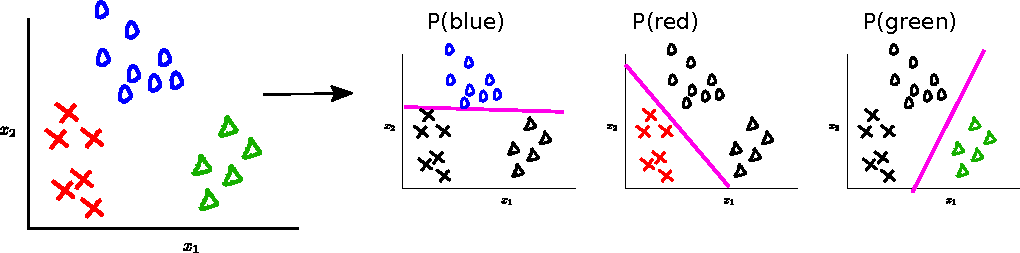
\includegraphics[width=0.9\linewidth]{MultipleClasses}
\caption{\footnotesize{\textbf{Logistic Regression multiple classes} Take all the training examples belonging to a specific class and now treat all of the other data as belonging to a single different class. So here our original classes are red, blue and green, but we treat it as three classification problems: red vs the rest, blue vs the rest, and green vs the rest. Each of the individual classifications allows us to calculate the probability of belonging to that specific class when a new data point is presented. }}
\label{Fig: Multiple Classes}
\end{figure}


\section{Overfitting and underfitting}

An underfitting model is said to have a \emph{high bias}, which refers to the algorithm having a very strong bias to use a particular model (e.g. a linear one in Fig. \ref{Fig: UnderOver}) regardless of the actual data. 

If we are overfitting we might be able to correctly predict each data point in our training set, but we have poor out-of-sample performance (Figure \ref{Fig: UnderOver}). A model that overfits is said to be \emph{high variance}. It can almost fit any function, the space of possible hypotheses is too large, too variable. 


\begin{figure}[h!]
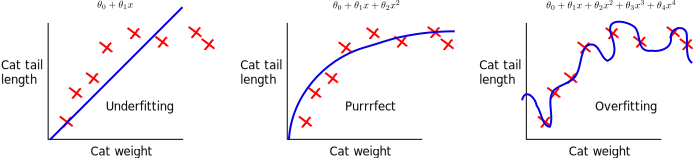
\includegraphics[width=0.9\linewidth]{UnderOver}
\caption{\footnotesize{\textbf{Under- and overfitting} The plots speak for themselves.}}
\label{Fig: UnderOver}
\end{figure}

\subsection{How do we know we are overfitting?}

One option would be to throw away some of the features, though this is not great because we're actually throwing away data. This is never good

Another option is regularization. We keep all the features but we reduce the magnitude of the parameters $\theta$. This works well when we have a lot of features, each contributing a little bit to our prediction $\hat{y}$.

\subsection{Regularization}

Suppose we do have some `complicated' linear regression model, i.e. $\hat{y} = \theta_0 + \theta_1 x + \theta_2 x^2 + \theta_3 x^3 + \theta_4 x^4$ and we want to find the optimal $\theta$. Using our normal cost function defined in Eq. \eqref{Eq: Cost function linear regression}, finding the optimal $\theta$ means minimizing $\sum_{i = 1}^m (\hat{y}_{\theta}(x\ind{i}) - y\ind{i})^2$. Now what if instead we penalize large values for the parameters $\theta_3$ and $\theta_4$ by adding terms to the cost function. For example, we can find the $\theta$ that minimizing the following expression:
\begin{equation}
\frac{1}{2m} \sum_{i = 1}^m \Big(\hat{y}_{\theta}(x\ind{i}) - y\ind{i}\Big)^2 + 1000 \, \theta_3^2 + 1000 \,\theta_4^2
\end{equation}

This will mean our model $\hat{y} = \theta_0 + \theta_1 x + \theta_2 x^2 + \theta_3 x^3 + \theta_4 x^4$ becomes more or less a quadratic function because the optimal $\theta_3$ and $\theta_4$ will be very small (assuming 1000 is large compared to the actual $x$ values used). 

The idea is as follows: small parameters $\theta_0, \theta_1, \cdots, \theta_n$ values lead to a simpler hypothesis and the model becomes less prone to overfitting. Now one may wonder why making \emph{all} parameters smaller still leads to a simpler hypothesis (clearly if we make the higher order terms smaller then yes our function is simpler, but if we make all of them smaller instead of specifically the higher order ones?), but this is true anyway. Just try. 

\subsubsection{Examples}
Suppose we have 100 features, $x_1, x_2, \cdots, x_{100}$ and we have 100 parameters $\theta_1 \cdots \theta_{100}$. As it is, we don't even know which parameters multiply higher order features (it may be e.g. that $x_5 = x_1^3$) so we cannot penalize only higher order terms even if we wanted to. The way in which we will modify the cost function is:
\begin{equation}\label{Eq: Regularized linear regression}
J(\theta) = \frac{1}{2m} \Bigg( \sum_{i = 1}^m \Big( (\hat{y}(x\ind{i}) - y\ind{i})^2\Big) + \lambda \sum_{i = 1}^n \theta_i^2 \Bigg)
\end{equation}
The last term is called the regularization term and it just adds a cost to having large values of $\theta$. All values of $\theta$ are regularized except for $\theta_0$ (that's a convention, it doesn't really make any difference). The parameter $\lambda$ is called the \emph{regularization parameter}. $\lambda$ controls the trade-off between fitting the training set well and keeping the parameters small. If $\lambda$ is too small we might overfit, if $\lambda$ is too large we will underfit as we fail to fit the training data (very high $\lambda$ leads to a prediction of $\theta_0$, so the `bias' of the cat tail length being $\theta_0$ is very high). Of course we know better, as baby kittens obviously have shorter tails than adult cats. 

If we were to use regularization on Figure \ref{Fig: UnderOver} then the graph on the right will look more to the one in the middle. It won't be completely quadratic, but the higher order terms will have a relatively lower contribution, it will basically become a wobbly version of the middle graph. 

\subsubsection{Regularized linear regression}

Our cost function is given by Equation \eqref{Eq: Regularized linear regression} and we update our parameters $\theta$ using the rule
\begin{align}
\theta_k &\rightarrow \theta_k - \frac{\alpha}{m} \Bigg( \sum_{i = 1}^m (\hat{y}(x\ind{i}) - y\ind{i}) \, x_k\ind{i} + \lambda \theta_{k} \Bigg) \nonumber \\
&= \theta_k \left(1 - \alpha \frac{\lambda}{m}\right) - \frac{\alpha}{m} \sum_{i = 1}^m (\hat{y}(x\ind{i}) - y\ind{i}) \, x_k\ind{i} \label{Eq: Regularized theta update}
\end{align}
This can be trivially shown by calculating $\partial_{\theta_k} J(\theta)$. Note that the above equations only hold for $k \neq 0$, when $k =0$ the term with $\lambda$ is dropped because $\theta_0$ is not regularized. 

The term $\left( 1 - \alpha \frac{\lambda}{m} \right)$ is usually quite close to one (if e.g. many training examples $m$ and a small learning rate $\alpha$). So the effect is that instead of just $\theta_k$ as the first term (as in Eq. \eqref{Eq: Theta update rule}) we use something like $0.99 \theta_k$. So on every iteration the parameters $\theta_k$ are shrunk a little bit and then the `normal' update term is added (i.e. the $- \alpha \sum$ etc..).

The normal equation also changes when we use regularization, it becomes:
\begin{equation}
\theta = \left( X^T X + \lambda \begin{pmatrix}
0 & 0 & 0 & \cdots & 0 \\
0 & 1 & 0 & \cdots & 0 \\
0 & 0 & 1 & \cdots & 0 \\
\vdots & \vdots & \vdots  & \ddots & \vdots \\
0 & 0 & 0 & \cdots & 1
\end{pmatrix} \right)^{-1} X^T y
\end{equation}
The derivation of this is shown in XXX. The matrix is a $(n + 1) \times (n + 1)$-dimensional matrix.

\subsubsection{Non-invertibility}\label{Sec: Regularization and invertibility}
Suppose that $m \leq n$, i.e. our number of training examples is less than the number of features. In this case, the matrix $X^T X$ is non-invertible. However, if $\lambda > 0$ then because we now take the inverse of $(X^T X + \lambda \cdot \text{Matrix})$ and that matrix \emph{is} invertible. So regularization takes care of any non-intvertibility problems of $X^T X$!.

 
\subsubsection{Regularized Logistic Regression}

Our non-regularized cost function for logistic regression is provided in Eq. \eqref{Eq: Final Final logistic cost function}, the regularized cost function has an additional term which is exactly the same as the term we added for linear regression, i.e. $\frac{\lambda}{2 m} \sum_{j = 1}^n \theta_j^2$. So again, all we do is add a term which penalizes large parameter values. The update rule for $\theta$ is again given by Eq. \eqref{Eq: Regularized theta update}, with the only difference that now $\hat{y}(x\ind{i})$ is a logistic function whereas for linear regression is was a linear function (just like Eqs. \eqref{Eq: Unregularized theta update rule} and \eqref{Eq: Theta update logistic unregularized} were the same). This of course makes a lot of sense as we wrote things down in a general way.

\section{Neural Networks}
Why do we want to use neural networks? In many problems, e.g. when recognizing images, the number of features can be very large. For example, a 200 by 400 pixel image already has $200 \times 400 \times 3 = 240000$ features (the 3 because of RBG), and that's only the actual pixel values themselves. If we want to fit a model that is nonlinear, we would need to take nonlinear combinations of features, e.g. $x_1 x_2, x_1 x_2^2, x_3^2$ etc.. (which is what we did to be able to separate the classes shown in Figure \ref{Fig: Logistic regression}C. With so many features, linear or logistic regression is not a good option. 

Neural networks were developed to simulate actual neural networks in the brain. Figure \ref{Fig: Neuron}A,B shows a cartoon of actual neurons and their (basic) neural network representation. This figure just shows one layer, but we can have more (Figure \ref{Fig: Neuron}C). Anything that is not an input or output layer is called a `hidden layer'.

As shown in the figure, the notation $a\ind{j}_i$ denotes the activation of unit $i$ in layer $j$. This is just the output value of that particular unit and goes along the axon to neurons in the next layer where the signal is combined with other incoming signals (in a weighted manner, as the synapses carry weight) and then this combined weighted signal goes through the activation function of these next-layer neurons. Each of the neurons in the next layer has its own weights so even though they all receive the same inputs, their outputs will generally be different. 

The activations in Figure \ref{Fig: Neuron}C are calculated as follows:
\begin{align}
a\ind{2}_1 &= g(\theta\ind{1}_{10} x_0 + \theta\ind{1}_{11} x_1 + \theta\ind{1}_{12} x_2 + \theta\ind{1}_{13} x_3) \nonumber \\
a\ind{2}_2 &= g(\theta\ind{1}_{20} x_0 + \theta\ind{1}_{21} x_1 + \theta\ind{1}_{22} x_2 + \theta\ind{1}_{23} x_3) \nonumber \\
a\ind{2}_3 &= g(\theta\ind{1}_{30} x_0 + \theta\ind{1}_{31} x_1 + \theta\ind{1}_{32} x_2 + \theta\ind{1}_{33} x_3) \nonumber \\
\hat{y}_{\theta}(x) &= a\ind{3}_1 = g(\theta\ind{2}_{10} a\ind{2}_0 + \theta\ind{2}_{11} a\ind{2}_1 + \theta\ind{2}_{12} x_2 + \theta\ind{2}_{13} x_3) 
\end{align}
with $g()$ the activation function which can e.g. by the sigmoid we used previously, $g(z) = 1/(1 + e^{-z})$. In this example, $\theta\ind{1} \in \mathbb{R}^{3 \times 4}$ and $\theta\ind{2} \in \mathbb{R}^{1 \times 4}$ meaning we have a single output neuron which itself received four inputs. The indexing is perhaps a little confusing as terms like $\theta_{00}$ don't really exist, which is just because the $0$ units don't have an input themselves, they are biases and their output is always 1. 
In general, if a network has $s_j$ units in layer $j$, and $s_{j+1}$ units in layer $j + 1$, then $\theta\ind{j} \in \mathbb{R}^{s_{j + 1} \times (s_j + 1)}$ (note that the $0$ units do not count as a unit when counting the number of units in layer $j$, so in the example in Figure \ref{Fig: Neuron}C we have three units in both layer 1 and 2).

\begin{figure}[h!]
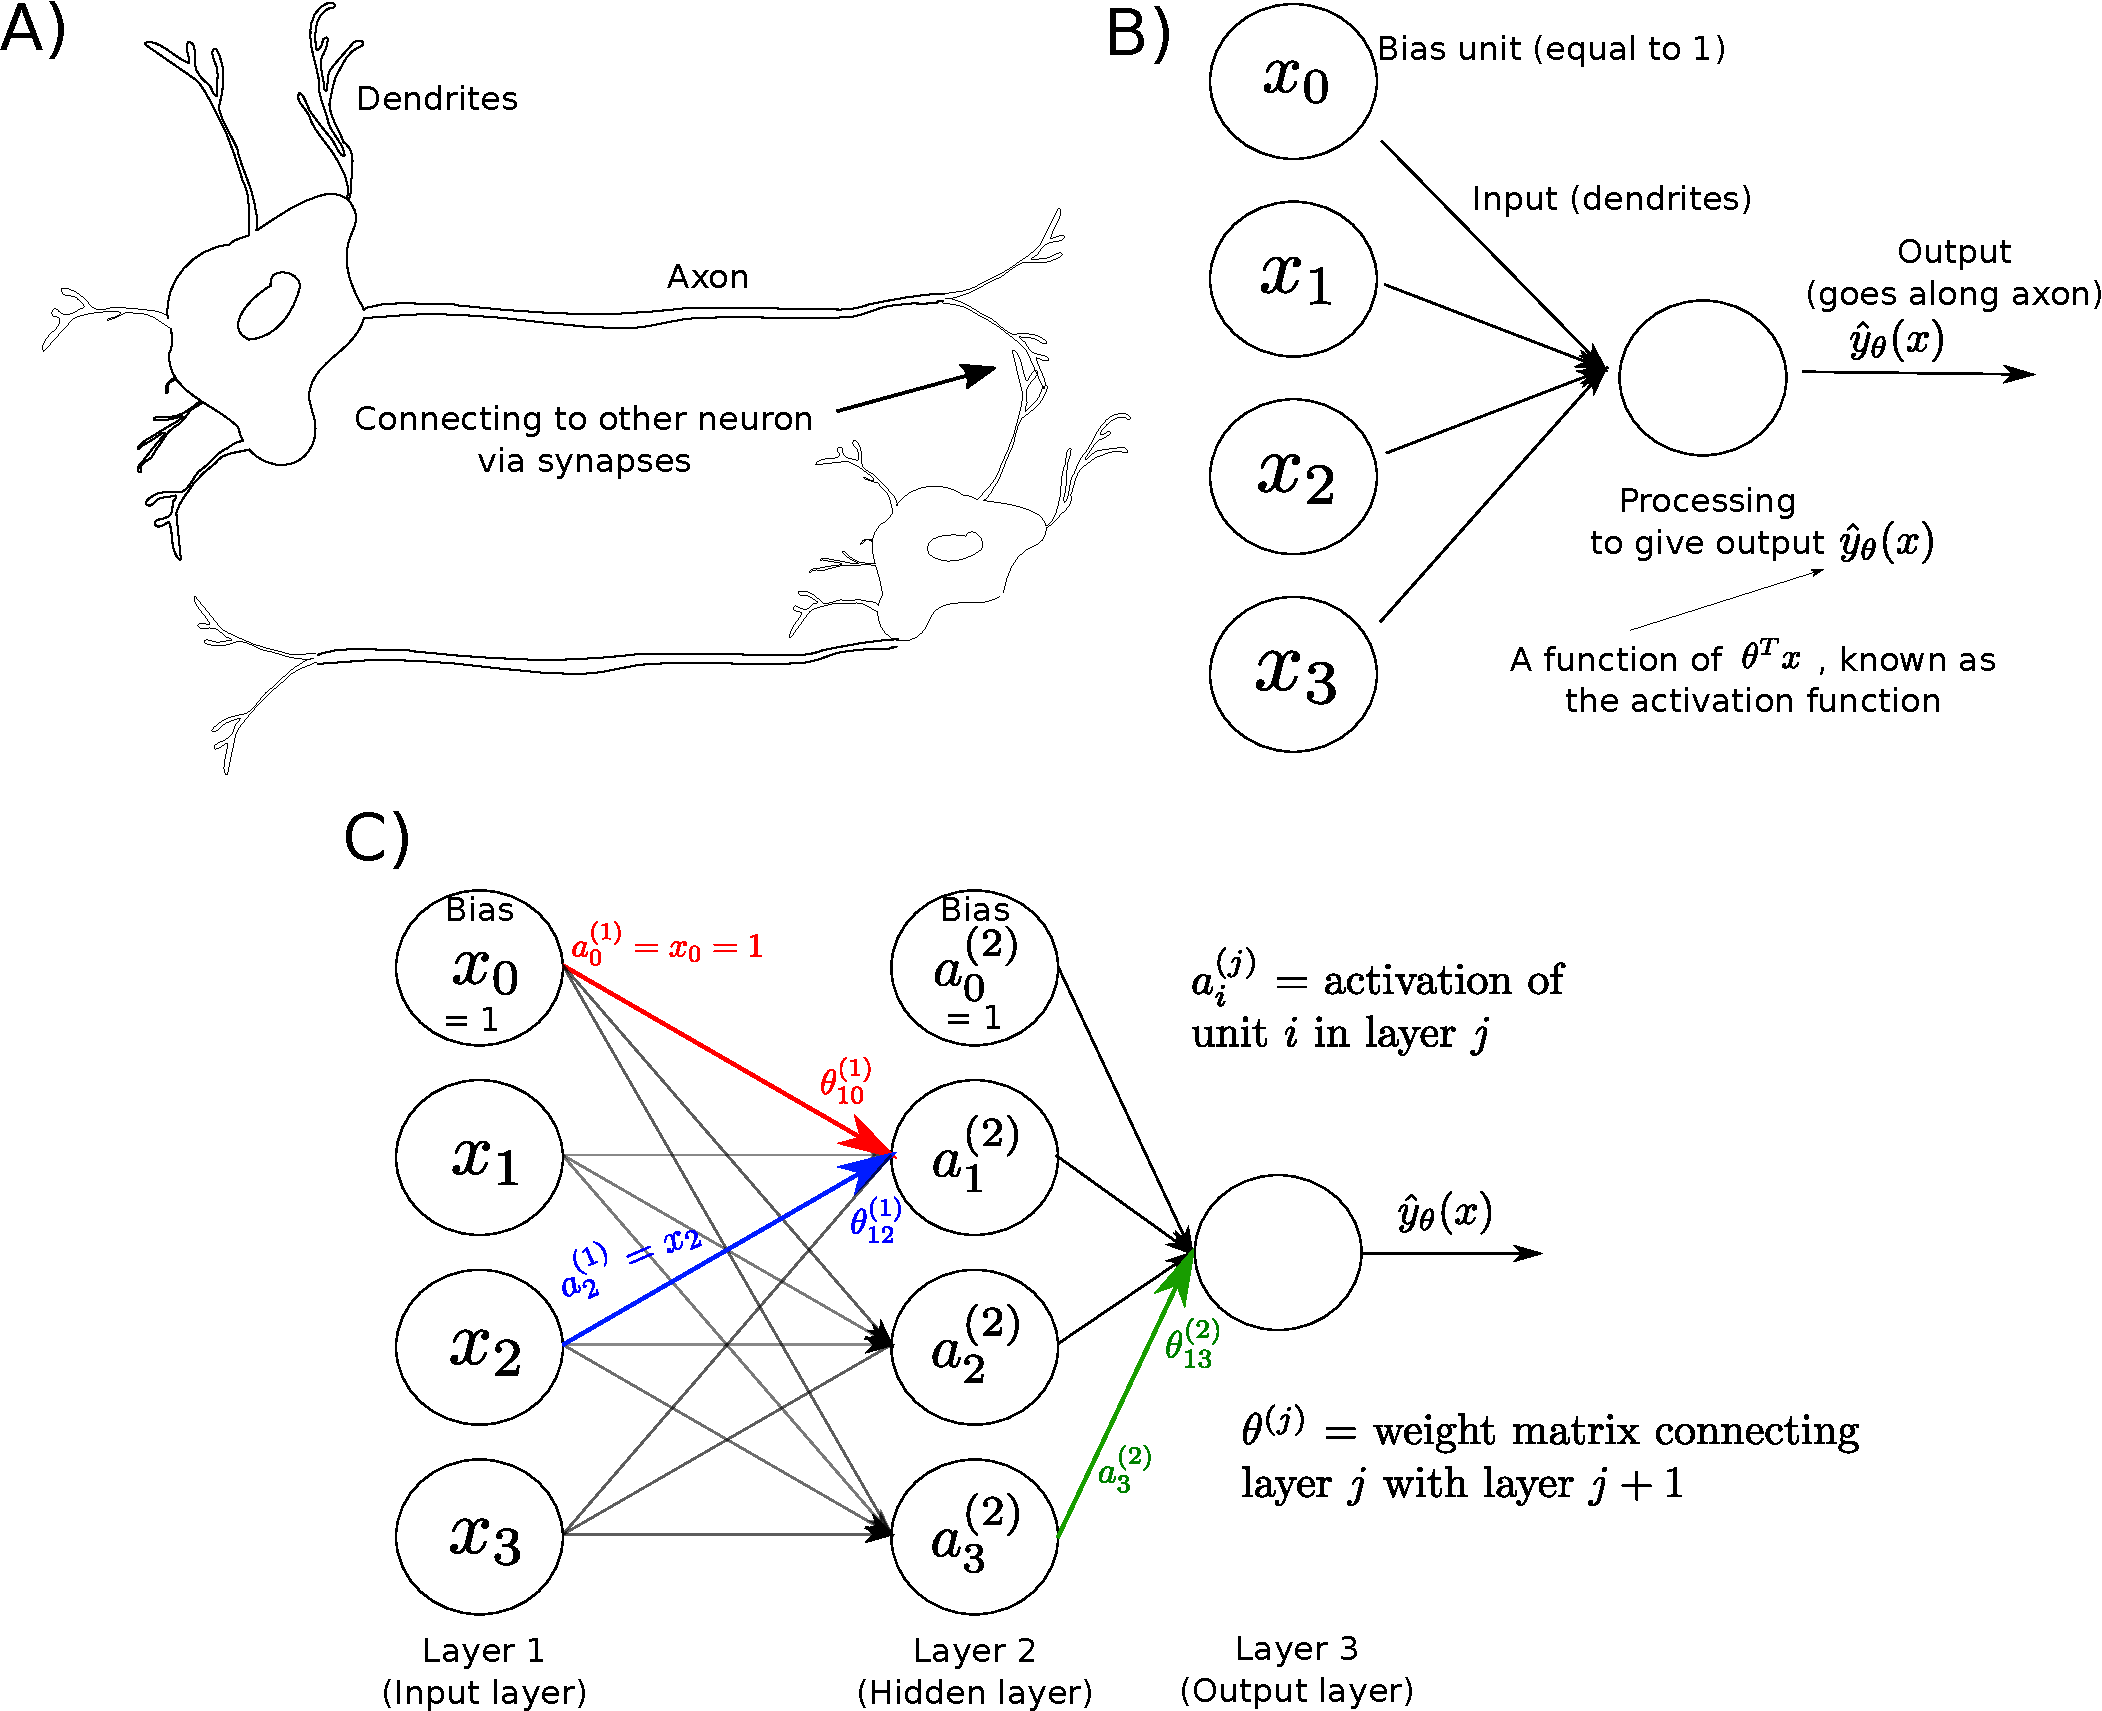
\includegraphics[width=0.9\linewidth]{NeuralNetwork}
\caption{\footnotesize{\textbf{Neural network representation A)} A cartoon of actual neurons. \textbf{B)} The basic units of a neural network and their relation to actual neurons. \textbf{C)} An example of a neural network with a single hidden layer and a single output neuron. }}
\label{Fig: Neuron}
\end{figure}

We can write the above example in a more compact form, namely 
\begin{align}
a\ind{2} &= g(\theta\ind{1} a\ind{1}) \nonumber \\
a\ind{3} &= g(\theta\ind{2} a\ind{2})
\end{align}
so we get
\begin{equation}
a\ind{i} = g(\theta\ind{i-1} a\ind{i - 1})
\end{equation}


\subsection{Some intuition}
The output neuron does its processing in a similar way as logistic regression, in inputs are now not $x$ and $\theta$ but the activations $a\ind{2}$ and $\theta$. So it's like the neural network still does logistic regression (as its final answer basically) but it chooses its \emph{own} features to use rather than simply using the input values $x$. You can get some complex features (i.e. complex combinations of the $x$ values) by having these $\theta$ matrices. The more hidden layers, the more weird combinations and weighting etc.. we can make from the intputs $x$. So neural networks `create their own feature vectors' on which they then perform logistic regression (well, if we use the sigmoid as the final activation function). Of course the output layer can be more than just a single neuron, but the intuition remains the same. 


\subsection{Forward propagation}



\subsection{Back propagation}

%https://machinelearningmastery.com/implement-backpropagation-algorithm-scratch-python/

\section{How to improve}
If you've implemented a machine learning algorithm, you've trained it but then when you test it on other samples (which were not in your training data) it turns out to perform very badly. What do you do?

There are diagnostic tests you can run, which can prevent you from wasting time on trying to improve your algorithm in a way that isn't fruitful. For example, sometimes more trainig data does not help and you are wasting time by trying to collect more data. A diagnostic test may tell you in advance that finding more training data is unlikely to be helpful.


\subsection{Training, (cross) validation and test sets}
You might need to chose whether to fit a linear function, quadratic, cubic, etc.. when you are using e.g. linear or logistic regression. One could fit all models to the training data to obtain, for each model, parameters $\theta\ind{d}$ were $d$ denotes the degree of the polynomial that was used to get that parameter estimate. 

One can then calculate the error of the models on a test set, and pick the model with the lowest test set error. Now we want to ask how well this picked model generalizes. To do this, one can NOT look at the error on the test set, because the value of $d$ was chosen already using the test set data. The test set error is likely to be an overly optimistic estimate of the generalization error. This is why we split in training, validation and test (instead of just training and test). It's typical to divide the data (0.6, 0.2, 0.2) between training, validation and test sets. 

To select our polynomial degree, we use the validation set to select the $d$ with minimum error (so minimum validation error). Then to get the generalized error of that particular polynomial we use the test set. 

\subsection{Over- and underfitting}
As shown in Figure \ref{Fig: UnderOver}, we might overfit (high variance) or underfit (high bias) our model. From Figure \ref{Fig: OverUnder Diagnostic} we see that we are likely to be \emph{underfitting} if $J_{\text{train}}(\theta) = \text{high}, J_{CV}(\theta) \approx J_{\text{train}}$ (where $J_{CV}(\theta)$ is the error using the cross-validation set). We are likely to be \emph{overfitting} if $J_{\text{train}}(\theta) = \text{low}, J_{CV}(\theta) \gg J_{\text{train}}(\theta)$


\begin{figure}[h!]
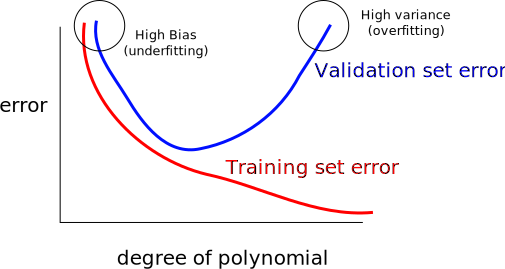
\includegraphics[width=0.6\linewidth]{OverUnder_Diagnostic}
\caption{\footnotesize{\textbf{Diagnostic for over- and underfitting} By comparing the errors from the training and validation sets, one can determine whether it is likely that we're over- or underfitting.}}
\label{Fig: OverUnder Diagnostic}
\end{figure}

\subsection{Choose the regularization parameter $\lambda$}
One can use the same method we used for determining what degree polynomial to use. Basically, use the model with the lowest validation error. 

Create some range of values of $\lambda$, e.g. $\lambda = 0, 0.01, 0.02, \cdots, \approx 10$. For each of these models, obtain the parameter fit $\theta$. Using these fitted $\theta$ values, calculate the errors using the cross validation set and pick the model with the lowest cross-validation set error. We can then obtain the test set error of that particular model to get an idea of the out-of-sample performance. 

When plotting the training and validation errors against $\lambda$, we get a something similar to Figure \ref{Fig: OverUnder Diagnostic}. The training error will increase with $\lambda$, the cross validation error will first decrease and then increase. Overfitting occurs at very small $\lambda$, underfitting occurs at very large $lambda$.

\subsection{Learning curves}
A learning curve is a plot of the training and cross validation errors as a function of the size of the training set (i.e. the number of training examples).

When you have high bias (underfitting) more training data does not improve your errors, whereas when you're overfitting more data does decrease your validation error (Figure \ref{Fig: Learning curve}). 

Learning curves are useful to again get a better idea of whether we are over- or underfitting and whether collecting more data would help.

\begin{figure}[h!]
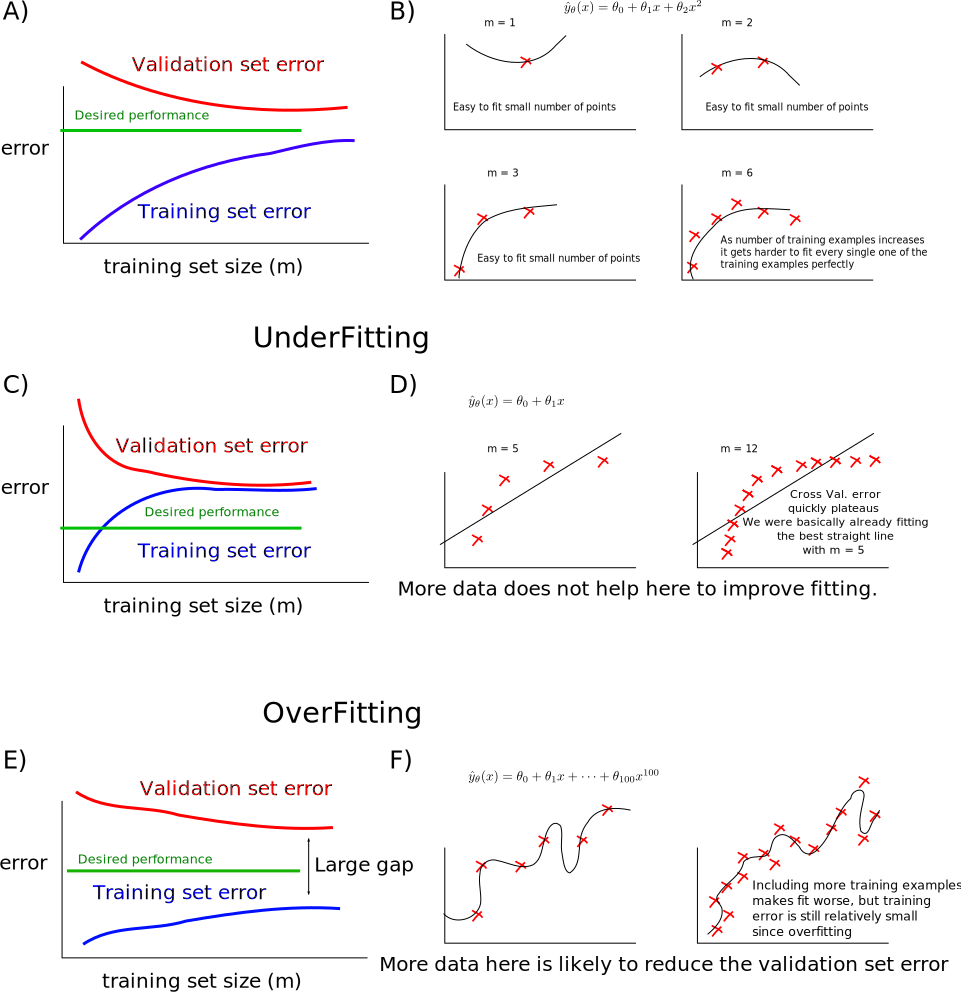
\includegraphics[width=0.9\linewidth]{LearningCurve}
\caption{\footnotesize{\textbf{Learning curve} Here we compare learning curves in  `good' (A,B), underfitting (C,D) and overfitting (E, F) scenarios. The figures on the right are meant to motivate some of the shapes of the learning curves on the left. }}
\label{Fig: Learning curve}
\end{figure}


\subsection{So, what do we do?}


\begin{table}[h!]
\centering
\begin{tabular}{|p{5.5cm}|p{7.5cm}|}
\hline
Option & When useful \\
\hline
\hline
Getting more training examples & This can help fix overfitting (high variance) \\[0.05cm]
\hline
Try smaller sets of features & This can help fixing overfitting (high variance). There is no point in carefully selecting a smaller set of features when you are underfitting.\\[0.05cm]
\hline
Try getting additional features & Usually this could help fix underfitting (high bias)\\[0.05cm]
\hline
Try adding polynomial features ($x^2_1, x^2_2$, etc) & Can help fixing underfitting (high bias)\\
\hline
Try decreasing $\lambda$ & Can help fixing underfitting (high bias) \\[0.05cm]
\hline
Try increasing $\lambda$ & Can help fixing overfitting (high variance) \\
\hline
\hline
\end{tabular}
\caption{\footnotesize{\textbf{Overview of when to use certain methods to improve performance} There are several ways in which the performance of our model can be improved, some are listed here. We also describe the situations in which these `improvements' would or wouldn't work. }}
\label{Tab: Improving performance}
\end{table}

When using neural networks, a small network is nice because it is computationally cheaper but it is prone to underfitting. Larger networks are more computationally expensive and can be prone to overfitting. Regularization can be used to reduce overfitting. You can try to use several neural networks, each with a different number of hidden layers, then pick the one with the smallest cross-validation error. 

\subsection{Good way to start}
A good way to start a new project may be to
\begin{itemize}
\item Create a quick and dirty model that runs without errors, check the accuracy on the cross-validation set
\item Plot learning curves, etc.. to find out whether the  model may be over- or underfitting. Improve if necessary
\item Look at some examples it got wrong and see you can come up with better features. Look at some examples that it got correct. You might find that some features didn't really help in getting the images correct, those could e.g. be dropped (if you want to drop features).
\item If there's a fast way of checking whether including something new (like `stemming' which can treat words like 'discount', 'discounts', 'discounted' etc.. as the same word, which might be useful in natural language processing) then you can just compare the cross-validation error with and without this new feature and see whether it's worth using it.
\end{itemize}


\subsection{Skewed classes}
Suppose you want to determine whether a change you just made to your model is actually an improvement. You look at the cross-validation error and the error has reduced from 0.8\% to 0.5\%. Great! Or not? If one class is much more represented than another, then it can be hard to determine whether the change has actually improved the model by merely looking at a single number. 

For example, suppose we are creating a model for breast cancer classification in which we want to predict whether or not someone has breast cancer, but only 0.5\% of the samples in our validation set correspond to someone having breast cancer. Then a classifier that always predicts no cancer only has a 0.5\% error. This means that if we changed our model to only predict `no cancer', we also would have reduced our error from 0.8\% to 0.5\% but it would obviously be a bad change. Basically, when the classes are skewed it could be that your lower error is `accidental' and does not really reflect whether an actual improvement was made or not. So what do we do in this case?

One good option is to look at the \emph{precision} and \emph{recall}. The precision is the number of true positives divided by the number of predicted positives, which is also just $true\,pos / (true\,pos + false\,pos)$. Suppose we classify whether a person has breast cancer or not, false positives would be when we tell someone he/she has cancer while they actually don't.

The recall is the fraction of all the actual positives that we actually classified as positives (which is $ true pos/(true\,pos + false\,neg)$. A high recall is good. In the example sketched above, our recall would be zero which immediately tells us that the classifier is bad. Note that our recall is only zero if we represent the underrepresented class as `1' (positive).

%Of course to visualise all these true/false positives and negatives we can plot the confusion matrix. If both the precision and recall are high, then the model is probably quite ok.

Supose we only want to tell people they have cancer when we are 70\% sure they actually have cancer. In a logistic regression model, this would mean predicting `1' if $\hat{y}_{\theta}(x) \geq 0.7$ and `0' otherwise (instead of setting the threshold at $0.5$. This will increase the precision but lower the recall. Similarly, setting the threshold lower than $0.5$ leads to higher recall and lower precision. Which one you want to be higher depends on the individual problem. When the threshold is at $0.5$ our recall and precision have a more intermediate values. 

The disadvantage of only looking at the precision (P) and recall (R) is that now we have two numbers. Is it better to have a P and R of 0.5 and 0.4, to of 0.7 and 0.1? One way to combine precision and recall is called the \emph{$F_1$-score} (also known as the $F$-score):
\begin{equation}
F_1 = 2 \frac{PR}{P + R}
\end{equation}
Then pick the choice with the highest $F_1$-score. So one could pick a range of threshold, evaluate the cross-validation $F_1$-score and automatically pick the threshold with the highest score. In this way you don't have to manually tweak it or think about it too much. The $F$-score is just one particular example of choosing combining the precision and recall, there are many others. If a human can predict the answer, a machine could as well if it has access to enough training data (as humans are of course just trained `computers' themselves). 


\subsection{Does more data help?}

A study in 2001 showed that a bunch of different algorithms performed very similarly and their accuracy increased monotonically with the amount of training data. This suggests that even a `bad' model with a lot of data can beat a much better model with less data. This led to the saying 

\blockquote{\emph{`It's not who has the best algorithm that wins. It's who has the most data.'}}

 How do we know whether a problem can benefit from more data? If this is the case then we might want to spend more time collecting more data instead of perfecting the model.

On good indication is whether a human expert can confidently predict the correct output given the input. For example, suppose you want to fill in one of the words `too, two, to' in the following sentence: For breakfast, I ate $\cdots$ eggs. The correct answer is clearly `two'. However, if the problem is to predict the house price based on only its size, then even humans may not do this very well. There are many other factors (e.g. location, number of bedrooms, how modern it is, whether there is a garden) that determine house price. So in this case the features we have are actually not sufficient themselves to get the correct answer. 

If the features \emph{can} accurately predict the correct outcome, then  when we have a model with many parameters (which will have low bias) and a really large training set (which gives us low variance), we are in a good place. 

\section{Support Vector Machines}

\begin{itemize}
\item Adjusted (simplified) logistic regression
\item Slightly different formulation, use parameter $C$ instead of $\lambda$, is roughly corresponds to $1/\lambda$
\item SVMs do not give probabilities as outcomes (as linear regression models do do) but they just output the predicted class
\item Is also called a large margin classifier (which is technically only true if $C$ is very large)
\item If $C$ is very large, the decision boundary generated is very sensitive to outliers. Also if the data is not linearly seperable, a large value of $C$ doesn't work well (it really tries to fit the exact data and is not good at dealing with noise). A smaller $C$ is able to ignore outliers
\end{itemize}

\subsection{Cost function for SVM}

\subsection{Kernels}

One way we dealt with nonlinear decision boundaries is to create new features by creating a polynomial of the components of the input vectors. For example, if the original $i$th training example was a vector $x\ind{i} = (x\ind{i}_1, x\ind{i}_2, x\ind{i}_3)$, we create a new set of features, which we will call $f\ind{i}$, given by e.g. 
\begin{align}
f\ind{i}_1 &= x\ind{i}_1  && f\ind{i}_2 = x\ind{i}_2 \nonumber \\
f\ind{i}_3 &= x\ind{i}_3  && f\ind{i}_4 = x\ind{i}_4 \nonumber \\
f\ind{i}_5 &= (x\ind{i}_1)^2  && f\ind{i}_6 = (x\ind{i}_2)^2 \nonumber \\
f\ind{i}_7 &= (x\ind{i}_3)^2  &&f\ind{i}_8 = x\ind{i}_1 x\ind{i}_2 \nonumber \\
etc...
\end{align}
For each new training example $x$, we have a vector with all these feature values, then calculate the cost of that training example given our weights, do that for each training example to get the overall cost, adjust weights, etc.. 

Though we can get some complex looking decision boundary, polynomials are of course not the only (and it turns out not the best) way in which we might create a nonlinear function. One common way of creating new features is to use \emph{gaussian kernels}. The features now do not include the components of the training examples themselves anymore, but are formed by creating guassians around each of the sample vectors $x^{(i)}$ and evaluating the guassian function at each of the training examples. To make this more concrete, we obtain the following features:
\begin{align}
f_1\ind{i} &= e^{(x\ind{i} - x\ind{1})^2/(2 \sigma^2)} \nonumber \\
f_2\ind{i} &= e^{(x\ind{i} - x\ind{2})^2/(2 \sigma^2)} \nonumber \\
&\vdots \nonumber \\
f_m\ind{i} &= e^{(x\ind{i} - x\ind{m})^2/(2 \sigma^2)} 
\end{align}
Now the number of features we have is equal to the number of training examples. Each feature is a measure of the distance between the current training example and all the other training examples. Note that, for each training example $i$, one of the features will be equal to 1 ($f_i\ind{i} = 1$). Also, a feature $f_0\ind{i} = 1$ is added to represent the intercept (like $\theta_0$ previously), meaning that the feature vector is $(m+1)$-dimensional: $f\ind{i} \in \mathbb{R}^{m+1}$.  This is illustrated in Figure \ref{Fig: Gaussian Kernel}.

\begin{figure}[h!]
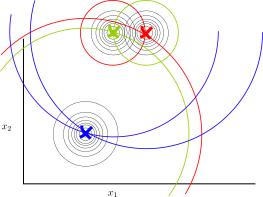
\includegraphics[width=0.6\linewidth]{GaussianKernel}
\caption{\footnotesize{\textbf{Gaussian kernel features} This cartoon illustrates how the features of a SVM with gaussian kernels are constructed. Consider the red training example. The features corresponding to this red example are the values of the gaussians centered at each of the training examples (including itself) at the position of the red example itself. These are indicated by the red circles (and the gaussian centered at the red example itself represents a feature value of $1$). The same is true for the other training examples. For example, if we denote the red, green and blue training examples by $x\ind{1}, x\ind{2}$ and $x\ind{3}$, then $f_3\ind{1}$ has a small value whereas $f_2\ind{1}$ is larger. Each training example here is represented by a $4$-dimensional feature vector. }}
\label{Fig: Gaussian Kernel}
\end{figure}

Similar as before, we will calculate the quantity $\theta^T f\ind{i}$ to determine which class to predict for intput $i$. If there are only two classes, we predict `1' if $\theta^T f\ind{i} \geq 0$. If there are more than two classes we can apply the 1-vs-all method in a similar manner as before (i.e. train $K$ SVMs where $K$ is the number of classes such that we get $K$ parameters vectors $\theta\ind{1} \cdots \theta\ind{K}$ and choose the class $j$ with the largest $(\theta\ind{j})^T x$ (for some training example $x$)).

We can also use kernels for logistic regression, but for logistic regression the algorithm then becomes very slow. SVMs are implemented in certain ways which makes them good for using kernels (I know this sounds a bit vague but it's just the way it is). 

If the parameter $\sigma^2$ is large, the features vary more smoothly as we update them because the slope of the gaussian at a certain distance from the centre is smaller compared to having a small $\sigma^2$. The model we fit with a large $\sigma^2$ tends to have a relatively high bias and low variance, and vice versa for a model with small $\sigma^2$.

To actually find the optimal parameters $\theta$, nobody really writes their own code to do this, there are researches who wrote libraries that numerically optimise this optimisation, so just use a library! Most packes have built-in multi-class classification so we can just provide it with the number of classes we have. So do we even need to do something ourselves? Well, we do need to make some educated guess for $C$ and the kernel (as well as the parameters that come with it). One can use the gaussian kernel described above, but also a linear kernel (which is basically `no kernel' and just e.g. calculates whether $\theta^T x \geq 0$) or some other kernel such as a chi-square kernel, string kernel, histogram intersectio kernel, $\ldots$. If the dimensionality of the inputs is large, a linear model might be better otherwise we could be overfitting. When using a gaussian kernel, e.g. if we have many training examples and the dimensionality of the inputs is relatively small,  we need to choose a $\sigma^2$. 

\subsection{Note on feature confusion}
The term `feature' is often use to denote an independent component of the training examples. Suppose we have a vector $x\ind{i} \in \mathbb{R}^6$ that is given to us, then we would say that there are 6 features. But then for the actual model training we can create additional features (or remove features). The eventual features we use for the training could be called `training features' which can include the `features' (as with logistic and linear regression) or not (with SVMs with a gaussian kernel). So don't be too confused whenever the word `feature' is used in slightly different settings. 

\subsection{Model selection tips}
Let $n$ denote the dimensionality of the input vectors that are given in some dataset, and $m$ the number of such vectors in the dataset. If $n$ is small and $m$ is intermediate, then it is good to use a SVM with Gaussian kernel. This could be e.g. when $n$ is roughly  $1 -  1000)$ and $m$ somewhere  between $(10 - 10000)$. If $n$ is small and $m$ is large (e.g. $n = 1 - 1000$ and $m = 50000 +$ then we might want to use logistic regression or a SVM with linear kernel and also increase the number of features (so let the `training features' be larger than $n$ by e.g. taking a high-degree polynomial with logistic regression). A neural network usually works well but may be slower to train.


\section{K-means clustering}

\subsection{The algorithm}


\subsection{How do we choose K?}
Unfortunately, there is no general method to determine the `best' value for K. One thing we can do is to maximise the Bayesian Information Criterion (BIC). The BIC is a criterion for model selection among a finite set of models. BIC penalises the use of more parameters as a model with many parameters can overfit the data and will, if its extra parameters are not penalised, always be the better model. The Akaike information criterion (AIC) can also be used. BIC penalises the number of parameters in the model more than AIC does. 
\begin{equation}
BIC(M | X) = k \text{log}(m)- 2 \mathcal{L}(X|M, \theta)
\end{equation}
where 
$\mathcal{L}(X|M, \theta)$ is the likelihood of the dataset $X$ given the model $M$ and parameters $\theta$, $k$ is the number of parameters in the model $M$, and $m$ is the number of datapoints we have. 

\section{Large data sets}
For very large data sets (e.g. hundreds of million or more training examples), using logistic or linear regression takes a long time. By plotting the learning curve we might find out whether using less training examples doesn't make much of a difference and we might just only use a subset of them (although I still have some feeling that throwing away data is throwing away information, which is always bad!). We here discuss some ways of dealing with big datasets. 

\subsection{Stochastic gradient descent}
For deterministic gradient descent, we compute the derivative of the cost function with respect to $\theta$ at each iteration. This means we need to sum over all training examples (see Eq. \eqref{Eq: Theta update logistic unregularized}) which will be very inefficient. This particular form of gradient descent is called \emph{batch gradient descent} because we use the whole batch (the set of training examples) to compute the derivatives. After all that work of calculating all these gradients, we have taken 1 step. We need to do that again and again and again. 



In stochastic gradient descent, we ..... %only look at a single training example. Instead of the cost function in like the one in Eq. \eqref{Eq: Cost function linear regression}, we would use $\frac{1}{2} (\hat{y}_\theta(x\ind{i}) - y\ind{i})^2$ without the sum over $i$.
Instead of first summing over all training examples and then taking 1 step, we just use a single training example and make a step (based on evaluating the derivative of the cost function but without looping over that $i$), then look at another training example and take a step, etc... Does the `stochastic' bit mean that we randomly pick the training example we want to use to evaluate the cost function, meaning that we might pick the same one multiple times in a row (theoretically)? ah no I think it's because we don't necessarily always move downhill so the trajectory towards the global minimum looks a bit random. It wanders around in the region close to the global minimum and doesn't necessarily stay there (since we're not optimising over all parameters simultaneously, we're doing it 1-by-1). \textcolor{red}{Don't really understand though, in the lecture slides he says that the number of steps we take like that to find the minimum is the same as the number of training examples so that suggests that indeed we just go through each of the training examples once. But wouldn't you want to maybe then go through it again, or indeed go through it randomly? Aaaah, ok the other repeat loop he has does exactly this. If do it multiple times we pass through the dataset multiple times. I think the outer repeat is the equivalent of the number of iterations in batch gradient descent.}% This whole process can then be repeated say 10 times or so (just like repeating the whole simulated annealing thing), also just to make sure that we consistently end up in the same location which then reassures us it's a global minimum (of course we start at different random initialisations of the parameter values each time). 

\subsection{Mini-batch gradient descent}
Stochastic gradient descent is in fact a form of mini-batch gradient descent with a batch size of 1, whereas batch gradient descent itself has a batch size of $m$ (all examples). In mini-batch gradient descent, as we might have expected, we use some batch size $1 < b < m$. Mini-batch gradient descent can be faster than stochastic gradient descent because we walk on the cost function space less randomly. Every step takes more time compared to stochastic gradient descent, but we walk towards the minimum in a more efficient way. Say e.g. you want to walk towards a house on top of a mountain and one path you can take is a nice paved road which goes around and around and is quite easy to walk on because it doesn't go up very steeply. So every step you take doesn't take a lot of effort, but you're getting to the house with a huge detour so in the end it might still take you a long time. Another path we can take is take a straight path up the mountain which means that we have to perhaps almost walk vertically at some points. Though the absolute distance we now travel is as short as it can be, it is very tiring and we'll probably fall to death or collapse due to exhaustion. A third path we might take has a decent slope so our calves will hurt after a while but it's manageable and we don't have to circle around the mountain as much as with the first path. Every step we take is more tiring compared to the first path but we take a more direct route and we might arrive sooner. Obviously there is a trade-off between the lenght of the path and the difficulty of the step and it probably depends on the cost landscape as well as the number of training examples what size of mini-batch is best.  Hmmmm, maybe this whole story is bullshit? He doesn't say anything like this. Ok apparently that trade-off doesn't really matter. If we have a mini-batch of $n$, then the step we take with the mini-batch thing is more or less equivalent of taking $n$ steps with the stochastic gradient descent because our step is indeed more directed. However, it takes $n$ times longer to compute because we sum over $n$ things instead of just taking 1. So in the end those things cancel out. The advantage of minibatch is now that we can do the $n$ steps in parallel (in stochastic gradient descent each new update has to be after the previous one as we used the newly updated theta to make the next step). Why then not just do batch gradient descent and parallelise the whole bunch? Apparently the step-size we take (which is basically this $n$) has some sort of upper bound depending on the smoothness of the objective function (something with the Lipschitz constant). I guess this makes sense, if the gradient changes a lot we can't just take one big step and expect to end up at the minimum. If the gradient of the objective function varies a lot we NEED to take smaller steps (this is basically saying that the learning rate cannot be very big) otherwise we might diverge, etc.. This link
%https://www.quora.com/Intuitively-how-does-mini-batch-size-affect-the-performance-of-stochastic-gradient-descent
explains it better and gives some intuition about what's numerically faster, etc.. That link also has a lot of answers to the question asked there from people who know much more about this than me obviously. It's good to read those things and understand a bit more about how to optimise things, how to think about computational efficiency, etc.. 

Mini-batch gradient descent generally only outperforms stochastic gradient descent if we have a nice vectorised implementation of our gradient descent which will allow you to partially parallelise the gradient computations over the $b$ examples. 

\section{Data compression}
Sometimes we might want to reduce the number of features in our dataset. We'll discuss some examples for 2D and 3D data because it's easier to interpret, but of course these ideas will then be generalised to much higher dimensional data. 

Suppose we have 2D data and want to convert this into 1D data. For example, we have two features which are highly correlated with each other. Though our data is 2D, it effectively lies in a 1D space, i.e. a line. We can represent each of the datapoints as just a single cooredinate, namely its position on the line. How do we choose this line? There are various ways of doing this, one of them is Principal Component Analysis, discussed below. 

A similar story holds for reducing 3D data to 2D data. If the 3D data actually lies roughly in a plane, we can project the data onto that plane. Then we only need two coordinates to determine the location of each of the datapoints on the plane. 


We might also want to use dimensionality reduction to visualise data. If we have 50D data and we want to reduce it to 2D in order to plot it, then some dimensionality reduction method can be used. Now what do the new two components mean? That's not always easy to interpret. By looking at which data point are plotted where in the space we may interpret the meaning of the two features ourselves. 

\subsection{Principal Component Analysis}
Principal Component Analysis (PCA) tries to find a lower-dimensional surface on which to project the data, while minimising the projection error. The projection error is often taken to be the sum of squared distances from the original data points to their projected locations. Before we do PCA, features should be normalised. 

%Note that PCA is not the same as linear regression. Suppose we have two features and we want to find the line to project the data on to reduce the dimensionality to 1D, we do not just fit a line using linear regression and use that line. With linear regression we find the line that 

In general we have $n$-dimensional data and we want to reduce it to $k$ dimensions. This means we have to find $k$ orthogonal vectors, $u\ind{1}, u\ind{2}, \ldots u\ind{k}$ which span the $k$-dimensional surface onto which the data is projected, while minimising the projection error.

We want to go from $n$ to $k$ dimensions.
First, we normalise the data for each feature, by subtracting the mean and dividing by the standard deviation (Eq. \eqref{Eq: Mean norm}).  Then, we compute the covariance matrix:
\begin{equation}\label{Eq: Cov matrix}
\Sigma = \frac{1}{m} \sum_{i = 1}^n \left(x\ind{i}\right) \left(x\ind{i}\right)^T
\end{equation}
and find the eigenvectors of this matrix. The covariance matrix is always symmetric positive semidefinite. Singular value decomposition (svd) can be used to get the eigenvalues (just use some library in whatever language we're using). Now we suppose that we have a matrix $U \in \mathbb{R}^{n \times n}$ whose columns represent the eigenvalues of $\Sigma$. Equation \eqref{Eq: Cov matrix} can be written in vectorised form as $\Sigma = 1/m X^T X$ with $X$ a matrix with each row representing a particular training example (i.e. $X \in \mathbb{R}^{m \times n}$. 

We can now pick the first $k$ columns of the matrix $U$, which we call $U_{reduce} \in \mathbb{R}^{n \times k}$. Then we calculate$U_{reduce}^T x = z$ which itself has dimension $(k \times n)\times (n \times 1) = k \times 1$. This vector $z$ is the $k$-dimensional vector we wanted. In these equations $x$ is just a particular training example, so if we label it by $x\ind{i}$ then we obtain $z\ind{i}$. 

\end{document}